\section{Terapia dei disturbi dell'umore}

Il \textbf{trattamento dei disturbi} dell'umore differisce in base al
tipo di disturbo che interessa il paziente, nonché in base alla sua
gravità, alle condizioni cliniche del paziente e dalla presentazione in
acuto o in cronico. Durante i trattamenti di emergenza è fondamentale
garantire la sicurezza del paziente valutando se vi siano le condizioni
per un trattamento ambulatoriale o se sia più opportuno il ricovero in
regime di day hospital o l'ospedalizzazione, anche mediante TSO, e
successivamente si può procedere con un'adeguata terapia farmacologica e
psicologica.

\subsection{Trattamento degli episodi depressivi}

\subsubsection{Linee guida}

\emph{\emph{CASO CLINICO: Nella fine degli anni '80 negli Stati Uniti un
nefrologo, dottor Osheroff, che dal punto di vista professionale ha
avuto un buon successo: ha un clinica importante, mentre dal punto di
vista sentimentale è al terzo matrimonio e mantiene in affido due figli,
avuti nei precedenti matrimoni.}}

\emph{Ad un certo punto comincia ad avere una sintomatologia depressiva
lieve, con una componente ansiosa piuttosto sfumata: chiede aiuto ad un
collega che gli prescrive una terapia farmacologica e una psicoterapia.
}

\emph{Fa la terapia in modo discontinuo, e dopo alcuni mesi si ritrova
nella situazione iniziale.}

\emph{Allora il suo collega gli propone un periodo di ricovero di alcune
settimane, così da poter tornare in seguito a fare la sua vita. Viene
ricoverato nel centro privato più prestigioso degli USA, dove la cura
fondamentale è la \textbf{psicanalisi}. Dopo il primo colloquio comincia
una terapia che consiste in quattro sedute a settimana, senza apporto
farmacologico.}

\emph{Dopo alcune settimane la situazione è peggiorata: non dorme, è
molto agitato, comincia a perdere di peso. Quando la moglie lo va a
trovare lui è preoccupato: la moglie, che lo è altrettanto, chiama un
collega psichiatra per confrontarsi sulla situazione. La clinica decide,
viste le perplessità, di riunirsi con il professionista esterno per
giudicare e poi decidere insieme il da farsi. Il responso della Case
Conference: ``la terapia è quella giusta, si tratta solo di aspettare
tempo''.}

\emph{Passano fino a sette mesi ed il paziente sta sempre peggio, è
dimagrito di 20kg, ha insonnia totale e compaiono anche deliri.}

\emph{La moglie allora dedice di trasferirlo da un'altra parte, in una
struttura che agisce con trattamento opposto, basato sull'approccio
farmacologico.}

\emph{Già dopo 2 settimane compaiono i primi miglioramenti. Trascorso un
mese e mezzo nella nuova clinica il paziente sta bene, è dimesso con
terapia da continuare da casa e altre sedute di psicoterapia.}

\emph{Tornato a casa dopo nove mesi il dottore, con centro di dialisi
chiuso e figli tornati dalla moglie, decide di fare causa alla prima
clinica (quella che basava l'approccio sulla psicoanalisi): chiede un
risarcimento danni, visto che non lo aveva curato per sette mesi.}

\emph{Il giudice ha chiesto a quelli della struttura i dati che avevano
a disposizione, per dimostrare che la terapia del dottore aveva dato
buoni risultati.}

\emph{Il problema è che gli psicanalisti hanno come posizione teorica il
fatto che la loro terapia non è misurabile, perchè quello che diventa
curativo è il rapporto che si instaura tra loro e il paziente, e quindi
è diverso da paziente a paziente; ciò diventa irripetibile, quindi
difficilmente misurabile.}

\emph{Per esempio esistono studi di meta analisi in cui si mettono
insieme tutti gli studi effettuati con la stessa metodologia, arrivando
ad avere risultati su casistiche molto ampie (anche 5000 pazienti).}

\emph{Perciò la clinica ha risposto che di risultati non ne avevano,
perchè per loro il metodo scientifico è inapplicabile alla psicanalisi.}

\emph{Il giudice prende atto e interpella la seconda clinica che ha
eseguito l'approccio farmacologico: loro hanno tutte le prove che
servono, perchè gli antidepressivi già dagli anni '60 erano usati e
dimostrati nella loro efficacia.}

\emph{Alla fine il giudice fondò la sua sentenza sul presunto silenzio
da parte della prima clinca (quella psicanalitica), riguardo gli effetti
postivi, scientificamente testati, della seconda clinca (quella con
trattamento farmacologico). Avrebbero dovuto avvisare il paziente della
possibile alternativa.}
\\\\
Non a caso che le prime linee guida, e quindi l' evidence based medecine
in ambito psichiatrico, sono uscite circa una decina di anni dopo,
proprio sul trattamento della depressione maggiore, per poi in seguito
uscire per tutti i disturbi.
\\\\
Su cosa si basa l'evidence based medecine?

Sono le metanalisi, degli studi clinici randomizzati in doppio cieco, ad
essere le più pesanti dal punto di vista dell'evidenza. Ci sono due
fattori fondamentali che deve avere il paziente per essere idoneo a uno
studio:

\begin{itemize}
\item
  non rimanere incinta durante la terapia: Abbiamo dati di trattamenti
  con antidepressivi in gravidanza, anche nel primo trimestre, che
  superano le 20000 pazienti, ma non sono stati mai approvati: andando a
  vedere le indicazioni del FDA (food and drug administration), non
  c'erano fino a pochi anni fa farmaci per il trattamento delle donne in
  gravidanza.
\item
  non essere a rischio di suicidio: se questo dovesse avvenire mentre
  assume un farmaco sperimentale, questo viene immediatamente
  abbandonato (ad esempio è successo a un farmaco della Pfizer per l'
  ipercolesterolemia).
\end{itemize}

Il problema che sorge da tutto ciò è il seguente: se non è possibile
mettere questi tipi di pazienti negli studi randomizzati, ma il medico
si trova a dover trattare uno di questi, non può rifiutarsi di trattarlo
perchè non sono presenti linee guida a riguardo. Risulta chiaro come sia
necessario agire ben oltre quello che è fornito dai dati statistici,
qualora, per necessità clinica, debba relazionarmi con una paziente
depressa incinta/ a rischio suicidio.
\\\\
\textbf{Dunque è per necessità clinica che le linee guide hanno dovuto
essere superate}. Quindi nelle condizioni cliniche rilevanti, in cui non
c'è uno studio che abbia trattato ad esempio un paziente a rischio di
suicidio, vale l'esperienza clinica.
\\\\
Come esempio:

\begin{itemize}
\item
  \emph{nei pazienti più gravi, in genere ricoverati, il fatto che io
  debba usare un triciclico non deriva dagli studi randomizzati, ma
  deriva esclusivamente dall'esperienza clinica.}
\item
  \emph{Nelle donne gravide: È bene precisare che farmaci
  anti-depressivi si usano anche nei primi trimestri di gravidanza e
  sono compatibili con l'allattamento, non perchè non passi (tutti i
  farmaci passano nella placenta e nel latte), ma la percentuale è
  davvero molto bassa. Qualche gruppo americano ha fatto anche un
  prelievo ai bambini ed era indosabile nel plasma.}
\end{itemize}

Di LINEE GUIDA ce ne sono tante, canadese, neozelandese, inglese ecc,
quelle forse migliori sono della \emph{American Psychiatric
Association}, perchè sono più approfondite, hanno più pagine su farmaci
e effetti collaterali. Quelle europee sono meno dettagliate, vi dicono
le indicazioni generiche per un determinato disturbo senza entrare nel
merito del singolo trattamento, quindi più in termini di scelta e durata
della terapia.

Per capire meglio, ad esempio le linee USA indicano per un trattamento i
possibili interazioni, effetti collaterali, mentre le europee non
considerano questi aspetti e danno linee di principio, infatti sono di
10-12 pagine contro le circa 100 delle altre.

\subsubsection{Indicatori nella scelta del trattamento}

Sono la Gravità e la Durata della depressione:

\begin{itemize}
\item[1.]
La GRAVITÀ della depressione:

  Per il DSM (Il Manuale Diagnostico e Statistico dei Disturbi Mentali)
  la \textbf{gravità dei sintomi} è espressa semplicemente contando il
  numero dei sintomi:

\begin{itemize}
\item
  lieve= 5,
\item
  moderata=7,
\item
  grave se maggiore di 7,
\item
  molto grave se ha sintomi psicotici, quindi depressione delirante.
\end{itemize}

  Questo è un criterio un po' grossolano, basta che ne abbia uno, ma
  molto intense, per avere un quadro più grave rispetto ad un altro:
  quindi tenere conto solo del numero, ma non della gravità, è
  estremamente impreciso.

  La depressione breve ricorrente ha i 5 sintomi, ha una durata molto
  più breve ed è, ad esempio, una forma con rischio di suicidio molto
  più elevato.

  Il ricovero dovrebbe scattare nelle forme deliranti, ad alto rischio
  di suicidio, o in forme molto complicate da gestire, ad esempio un
  anziano con problemi internistici.

\begin{itemize}
\item
  Per pazienti con una GRAVITÀ LIEVE le possibilità di trattamento sono
  molte:

Messa in evidenza in un grafico di meta analisi \textbf{l'efficacia
degli antidepressivi in relazione alla gravità della depressione,}
pubblicato su Jama.

Immaginiamo un grafico con\textbf{:}

In ordinate è espresso il cambiamento rispetto a prima del trattamento

In ascissa si trova la misurazione della gravità della depressione con
la scala di Hamilton. È da tenere presente che quando è svolto uno
studio su un nuovo farmaco in genere sono inclusi pz che abbiano almeno
18. Questo è il cambiamento che è possibile ottenere prima e dopo;
quindi se è ottenuto 12 vuol dire che c'è stata una riduzione di 12
punti della scala di Hamilton.

\textbf{Conclusioni ottenute:}

È stabilito a 25 il punteggio di gravità della sintomatologia
depressiva, misurata con il famoso Hamilton, che discrimina tra
superiorità del trattamento con farmaci rispetto al placebo.

Al di sotto di quel livello placebo e farmaci danno lo stesso risultato,
mentre al di sopra di 25 il farmaco è decisamente più efficace.

Diversi studi dimostrano che un punteggio inferiore a 23, quindi siamo
nella fascia sotto quel limite, è posseduto dai 2/3 (75\%) dei pazienti.

Quindi possiamo somministrare:

\begin{itemize}
\item
  PLACEBO: \textbf{Come dare un placebo al paziente:} È presa in esame
  una di quelle donne che tra i 15 e 50 anni vanno dallo psichiatra: ha
  una depressione di 24; si dimostra di poterle dare qualunque
  trattamento, ma come si fa a darle un placebo?

  Si potrebbe dare un antidepressivo, ma un conto è dirle che funziona
  come antidepressivo ed un conto è dire che funziona come placebo.
  Infatti, dicendole che è un placebo, praticamente non si riesce a
  somministrare un placebo, questo è difficile da applicare in
  psichiatria.

  È possibile allora dire alla paziente che il farmaco che assume non ha
  nessun effetto a livello farmacologico, ma attiva le stesse aree a
  livello cerebrale del farmaco vero e proprio, questo è stato il metodo
  per somministrare il placebo.

  Un americano lo ha fatto nel colon irritabile, il risultato è che
  l'effetto sulla patologia è analogo tra antiinfiammatorio e placebo.

  Prendendstudio sull'agopuntura per meglio descrivere l'entità
  dell'effetto placebo.

  Lo studio è sul trattamento di emicrania, cefalea muscolo tensiva,
  dolore lombare cronico, randomizzati. La usual care riceve visita
  medica più analgesico, l'altro gruppo è trattato con agopuntura:
  l'effetto è il medesimo.

  Inoltre nell'ambito della stessa agopuntura, far inserire gli aghi a
  un esperto agopunturista in punti ben determinati, oppure a una
  persona qualunque, purchè gli si insegni il metodo per inserirli,
  dimostra che il miglioramento del dolore è esattamente lo stesso.

  Se l'analgesico viene presentato dicendo che è il migliore farmaco,
  questo ha un effetto assolutamente migliore. Se lo stesso farmaco è
  somministrato endovena senza essere enfatizzato al paziente l'effetto
  analgesico scompare. Addirutta ci sono studi sul colore del farmaco
  placebo: più colorato è, meglio è efficace.

  In conclusione: l'aspettativa che ha il paziente assume un ruolo
  determinante nell'efficacia di un trattamento, sia che questo sia
  farmacologico, sia che sia un placebo.

  Quindi che il placebo sia una sostanza inerte, non è del tutto vero:
  il placebo modifica le aree cerebrali, cioè le stesse che modificano i
  farmaci; lo stesso fa la psicoterapia.

\item
  TERAPIA FARMACOLOGICA
  
\item
  TERAPIA PSICOTERAPEUTICA, di quest'ultime è dimostrata l'efficacia
  solo se ad orientamento cognitivo comportamentale.

  Il punto cardine di quest'ultime è: ``Io ho appreso qualcosa di errato
  che devo disapprendere''.

  Esempio: \emph{non avere sicurezza, non valere nulla, temere che tutto
  debba andare male;} è uno stile cognitivo che ho imparato e che devo
  disimparare.

  \textbf{Man mano che aumenta la gravità la psicoterapia perde
  efficacia,} la farmacoterapia diviene allora un'indicazione
  fondamentale.
\end{itemize}

È chiaro che bisogna ricordare quello che dicevano gli inglesi:
\textbf{tanto più il disturbo è lieve e breve, tanto più risponde alla
aspettativa di un miglioramento, qualunque esso sia}. L'agopuntura,
l'omeopatia, la terapia di rilassamento. Per l'omeopatia è uscito anche
un articolo sull'ansia assolutamento sovrapponibile al placebo.

\textbf{I triciclici in genere servono per le forme più gravi e il
placebo per quelle più lievi}. L'efficacia sale per tutti e tre i
trattamenti, placebo compreso, dagli anni '80 agli anni 2000.

Dagli anni '80 agli anni 2000 la risposta al trattamento è aumentata;
nel placebo va dal 20 al 30\%, mentre per i serotoninergici e
tricliclici dal 40 al 50\%.
\\\\
\emph{\emph{Quando uno psichiatra decide di somministrare a un paziente
con depressione lieve un trattamento farmacologico, deve tenere presente
che questo è analogo al placebo o al trattamento psicologico.}} Quindi
non c'è differenza di mortalità tra placebo e un farmaco normale nelle
forme lievi, il placebo equivale alla psicoterapia.
\\\\
A livello economico è più costoso dare un placebo che un farmaco.
Infatti è da tenere presente che un'ora di psicoterapia costa 80-100
euro, mentre il farmaco antidepressivo più prescritto costa 6 euro al
mese (quindi con 100 euro è possibile fare 16 mesi di terapia
farmacologica).
\\\\
Dal punto di vista di uno psicoterapeuta è importante che abbia la
consapevolezza di poter guarire l'episodio depressivo soltanto se questo
non è grave (può farlo, perchè in quel caso tutti i trattamenti sono
equivalent). Quello che invece lo psichiatra può fare non è pensare di
risolvere il conflitto alla base della depressione maggiore o del
disturbo bipolare, ma fare in modo che il paziente non abbia più
ricadute.

È possibile trattare l'episodio e aumentare la consapevolezza,
soprattutto nei bipolari, che è presente un disturbo da gestire, che
bisogna seguire la terapia con regolarità e adottare un certo stile di
vita.

Questo non è secondario, perchè nel disturbo bipolare i pazienti che
seguono il trattamento e le visite hanno un rischio di suicidio
dimezzato rispetto a quelli che non lo fanno: per cui lavorare su questo
è importante, perchè è ridotto il tasso di suicidio del 50\%.

\item
  Per pazienti con GRAVITÀ ELEVATISSIMA:

L'ELETTROSHOCK è stato scoperto da un neurologo italiano negli anni
  30, Ugo Cerletti. I farmaci esistono dagli anni '50, prima non si
  sapeva cosa fare.

  \emph{Il professore cita, per comprendere pienamente la difficoltà dei
  trattamenti psichiatrici prima dell'avvento dei farmaci, ``Le libere
  donne di Magliano'' e ``Per le antiche scale'', libri di Mario Tobino,
  uno psichiatra che ha lavorato nell'ospedale di Lucca.}

  \emph{Egli descrive i pazienti che vengono inviati alle ``alghe'', una
  stanza piena di alghe dove il paziente veniva messo nudo, per evitare
  che si potesse fare del male.}

  \emph{Prima del trattamento farmacologico si ricorreva a:
  elettroshock, shock insulinico, shock cardiazolico, bagni con shock
  termico.}

  \textbf{L'elettroshock è il trattamento più efficace in depressioni di
  gravità elevatissima}, è lo stesso concetto applicato nella
  cardioversione, annullare tutti i potenziali di membrana con una
  corrente, cosicchè i neuroni ripartano in condizioni normali.

  Ancora oggi ci sono pazienti lo richiedono, perchè la loro descrizione
  è questa: ``Entravo con nessun altro pensiero, se non quello di farla
  finita, ed uscivo che stavo bene''.

  È eseguito in anestesia generale, si vede la crisi epilettica solo per
  il movimento del piede, il paziente è curarizzato. È utile solo in
  questi casi, non ha altre indicazioni, farlo senza è una malpractice:
  oggi è praticamente limitato ai gravi rischi di suicidio.

\item
  Per pazienti con DEPRESSIONE DELIRANTE:

  ANTIDEPRESSIVI con associati ANTISPSICOTICI sono raccomandati, se è
  presente sintomatologia delirante.


\item
  Per pazienti con DEPRESSIONE associata a PATOLOGIA CORONARICA:

  La depressione rappresenta un aumento di rischio di mortalità in
  pazienti con patologia coronarica.

  Se prendiamo in considerazione pazienti con sintomi depresssivi
  (pazienti sotto soglia, in cui il quadro clinico depressivo non
  raggiunge la soglia della diagnosi), perchè mai andrebbero trattati?
  \textbf{\emph{Perchè con sintomi depressivi si ha un rischio 1.7 volte
  maggiore di morire, rispetto ad un altro paziente con la stessa
  patologia cardiaca (non depresso).}}

  Più la depressione è lunga, più questo moltiplicatore del rischio
  aumenta:
\begin{itemize}
\item
  2 se meno di 6 mesi
\item
2.6 se più di 6 mesi
\end{itemize}

Diventa quindi importante anche ciò che è sotto soglia, perchè ha
un'influenza infausta sul decorso di tutte le patologie, soprattutto
quelle cardiovascolari.
\\\\
La depressione, anche molto sfumata, ha un effetto nefasto sul decorso
di tutti i disturbi medici e in particolare le malattie cardiovascolari.
\\\\
\emph{Viene mostrato il risultato di uno studio pubblicato su JAMA,
relativo alla probabilità di morte dei pazienti post infarto, con e
senza un trattamento psicoterapeutico a confronto.}
\\\\
Sono più di 1000 pazienti che hanno avuto un infarto. Valutando le linee
guida, non è detto di doverli trattare con la terapia farmacologia;
quindi è possibile approcciarli tranquillamente con la terapia
psicologica.

Questo studio ha un braccio in cui i pazienti hanno un trattamento
psicologico e un braccio in cui i pazienti hanno un trattamento
farmacologico.

Il gruppo di controllo è definito \emph{usual care}. In pratica il
paziente è sottoposto a visita cardiologica, fa un colloquio sulle
condizioni cardiache e in parte anche sullo stile di vita.

L'altro gruppo oltre alla visita cardiologica riceve una psicoterapia
cognitivo comportamentale.

I due strumenti di valutazione:

\begin{itemize}
\item
  (BDI) auto-somministrato, è il paziente che lo compila\emph{: In
  genere l'autovalutazione tende a dare un disturbo un pò più grave,
  cioè tende a sovra-stimare la gravità}
\item
  HRSD è il medico che lo compila: \emph{mentre la valutazione di un
  osservatore tende a ridurre questa gravità}
\end{itemize}

Il risultato è che si si ha un miglioramento in entrambi i casi della
depressione ed è qui sorge il problema: esistono due trattamenti che,
secondo le linee guida, sono entrambi efficaci per le depressioni lievi.
Però i farmaci riducono la mortalità e i nuovi rischi di infarto, mentre
la psicoterapia, pur essendo efficace nella depressione non agisce sul
versante cardiovascolare.

Allora perché gli antidepressivi funzionano anche sul cuore? Lo si deve
al fatto che loro sono anche anti-aggreganti piastrinici? Non esiste
ancora risposta a questo quesito.
\\\\
\emph{Cochrane}, ente privato che si occupa dei problemi sanitari (in
genere fa delle metanalisi o revisioni) ha effettuato uno studio a
riguardo. Gli studi di questa agenzia hanno 3 destinatari:

\begin{itemize}
\item
  pazienti
\item
  medici
\item
  amministratori sanitari
\end{itemize}

\textbf{Si è concluso che gli interventi psicologici nel loro complesso
non hanno mostrato efficacia sulla mortalità totale cardiaca}, benchè
mostrino una riduzione nei livelli di ansia e depressione nei pazienti
con cardiopatia coronarica; questa è in parte la spiegazione del perchè
anche con depressione subliminare vanno trattati.
\end{itemize}

\item[2.]
  E' introdotto oltre al criterio di gravità anche quello di
  \textbf{DURATA}:

  Il trattamento farmacologico antidepressivo, ovviamente rispetto al
  placebo, è indicato nei casi particolarmente gravi oppure di durata
  prolungata. Quindi un caso di non particolare gravità, ma di durata
  prolungata, può trovare questa indicazione: è il caso della
  depressione sotto soglia, anche detta minore.
\end{itemize}

\subsubsection{Farmaci antidepressivi}

\begin{figure}[!ht]
\centering
	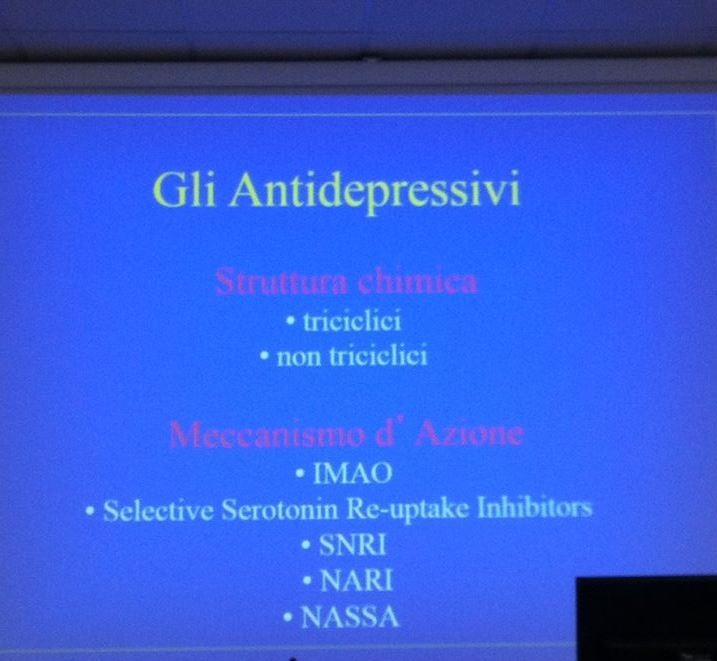
\includegraphics[width=0.9\textwidth]{03/image1.jpeg}
\end{figure}

Per gli \textbf{episodi} \textbf{depressivi}, il trattamento si basa
sull'uso dei \emph{farmaci antidepressivi} e, nei casi più gravi, della
\emph{TEC} (Terapia Elettro-Convulsivante); tra gli antidepressivi sono
disponibili diverse classi di farmaci, come gli \textbf{SSRI} (Inibitori
Selettivi della Ricaptazione della Serotonina), gli
\textbf{antidepressivi tetraciclici} e \textbf{triciclici}
(\textbf{TCA}), gli \textbf{IMAO} (Inibitori delle Monoammino-Ossidasi),
gli \textbf{SNRI} (Inibitori della Ricaptazione della Serotonina e della
Noradrenalina), i \textbf{NARI} (Inibitori Selettivi della Ricaptazione
della Noradrenalina), gli agonisti melatoninergici ed i \textbf{NaSSA}
(Antidepressivi noradrenergici e serotoninergici specifici).

\begin{itemize}
\item MECCANISMO:

\begin{itemize}
\item
  \textbf{Blocco del reuptake}:

  \begin{itemize}
  \item
    Serotonina (SSRI; SNRI)
  \item
    Noradrenalina (TCA;NARI)
  \end{itemize}
\end{itemize}

\begin{itemize}
\item[1.] ANTIDEPRESSIVI TRICILICI (TCA)

\emph{\emph{Usi Clinici:}}

I farmaci antidepressivi triciclici e tetraciclici (TCA) sono
generalmente riservati ai casi depressivi che \emph{non rispondono né
agli SSRI né agli SNRI}.
\\\\
In realtà sono farmaci di prima scelta per il trattamento delle forme
depressive di maggiore gravità: con \emph{caratteristiche melanconiche}
o con \emph{rallentamento motorio}; infatti quando prevalgono
l'inibizione ed il rallentamento è bene ricorrere a TCA ad azione
attivante, come la \textbf{desipramina} e la \textbf{nortriptilina}.
\\\\
Per le forme depressive \emph{con ansia ed agitazione} si utilizzano
preferibilmente l'\textbf{amitriptilina}, l'\textbf{imipramina} e la
\textbf{trimipramina}, che sono farmaci con marcata attività sedativa.
\\\\
Alcuni farmaci TCA, inoltre si sono dimostrati utili anche nel
trattamento di eventuali \emph{disturbi psichiatrici associati alla
depressione}, ad esempio:

\begin{itemize}
\item
  la \textbf{clomipramina} è utile per i pazienti depressi che soffrono
  anche di \emph{disturbo ossessivo} c\emph{ompulsivo}. infatti il
  disturbo ossessivo-compulsivo risponde esclusivamente ai farmaci
  serotoninergici o pro-serotoninergici, infatti con altri farmaci, per
  esempio ammine secondarie, non avviene la terapia. Tant'è che la
  clomipramina soltanto, perchè è aggiunto un cloro, è uno dei maggior
  farmaci che agisce sul sistema della serotonina. Dando altri
  triciclici non si nota nessun miglioramento; quindi solo modificando
  appena la struttura è ottenuta una diversa efficacia e tollerabilità.
\item
  mentre l'\textbf{imipramina} è efficace anche contro i sintomi del
  \emph{disturbo di panico.}
\end{itemize}

\emph{\emph{Effetti collaterali:}}

Gli \emph{effetti collaterali} dei TCA sono essenzialmente dovuti alla
loro azione anticolinergica, antistaminica ed adrenolitica, e sono
generalmente più intensi nelle prime due settimane di cura, con:
ipotensione ortostatica, tachicardia riflessa, turbe del ritmo e della
conduzione cardiaca, tremori, atassia, discinesie, deficit della memoria
e della concentrazione, sedazione e confusione (negli anziani), visione
offuscata, vertigini, abbassamento della soglia convulsiva, alterazioni
della libido, impotenza, ritenzione urinaria e, soprattutto nelle
terapie a lungo termine, aumento ponderale, stipsi, xerostomia ed
iperidrosi.

In particolare:

\begin{itemize}
\item
  \emph{Anti-alfa 1} -> Il tono delle arteriole dipende molto dalle alfa
  1, infatti i nostri pz hanno ipotensione ortostatica (in un giovane si
  annebbia la vista, mentre nell'anziano è più grave la situazione
  soprattutto se ha una placca emodinamicamente significativa come
  dicono i doppleristi)
\item
  \emph{Anti-H1} -> Aumento ponderale/ sedazione
\item
  \emph{Anti-muscarinici} -> in senso cranio-caudale causano alterazioni
  funzioni cognitive, glaucoma per aumento della pressione endo-oculare,
  lacrimazione, xerostomia (secchezza cavo orale quindi se deve parlare
  ve ne accorgete dopo un po di esperienza; se è anziano ed ha la
  dentiera è peggio), tachicardia (aumenta anche per l'ipotensione
  ortostatica), effetto sulla peristalsi e incontinenza urinaria
  (nell'anziano che magari ha anche la prostata va considerato).
\item
  \emph{Effetto chinidino simile:} A livello cardiaco non c'è tanto un
  effetto recettoriale (anti-muscarinico), ma un effetto
  chinidino-simile, come gli anti-aritmici di classe Ia; si ha
  allungamento del PR (se uno ha giù un blocco AV lo peggiora)
\end{itemize}

Eliminando la struttura triciclica questi effetti scompaiono; con la
rimozione di un gruppo metilico tra \emph{imipramina e desimipradina};
in questo modo calano effetti collaterali e c'è spostamento in termini
anche di efficacia farmacologica, che si sposta molto di più sulla
noradrenalina rispetto alla serotonina.
\\\\
Inoltre si deve sempre tenere a mente che \emph{l'indice terapeutico dei
TCA è basso}, circa 10 volte la dose massima consigliata, per cui si
corre un rischio non indifferente di sovraddosaggio, con
un'intossicazione acuta, fatale nel 15\% dei casi, in cui compaiono
midriasi, ipertermia, tachicardia, agitazione, confusione, convulsioni e
quindi coma.
\\\\
I TCA sono quindi \emph{controindicati} in: soggetti con glaucoma,
ipertrofia prostatica, infarto recente, insufficienza
cardio-circolatoria, disturbi del ritmo e della conduzione cardiaca.
\\\\
Per \emph{ridurre gli effetti collaterali} legati ai TCA, in genere si
comincia il trattamento con dosi di 25-50 mg/die, che sono poi aumentate
gradualmente di 25 mg ogni 2-3 giorni sino a raggiungere la dose media
di 150-250 mg/die in circa 10-15 giorni.
\\\\
Uscendo dalla struttura triciclica, c'è minore efficacia, ma migliore
bio-compatibilità (soprattutto a livello cardiaco e cardio-vascolare,
oltre a tutti gli altri effetti anticolinergici). Questi (classi di
farmaci a seguire) sono farmaci usati per depressioni non molto gravi,
in compenso migliora il proflilo di tollerabilità, avendo comunque
qualche effetto collaterale come nausea, agitazione.

\item[2.] \emph{2.SSRI}

Nei serotoninergici cambia radicalmente la struttura:

Sono farmaci non pericolosi ampiamente venduti : 300 mila
serotoninergici sono stati venduti per esempio nel 2015 in provincia di
Parma su una popolazione di 420 mila abitanti! Questo è un numero
esagerato, addirittura in Gran Bretagna sono 6 milioni di confezioni in
un anno.

Inoltre sono farmaci anche economici: una confezione per un mese di
citalopram costa 6 euro.

\emph{\emph{Usi Clinici:}}

Gli SSRI costituiscono la prima scelta nel trattamento della depressione
di lieve/media entità e nei casi in cui i TCA siano controindicati,
potendo peraltro essere associati con attenzione ai TCA o ad altri
antidepressivi in caso l'altro farmaco, da solo, non si riveli efficace
nel controllo dell'episodio.

\emph{\emph{Effetti collaterali:}}

I principali effetti collaterali degli SSRI sono l'inappetenza, il
dimagrimento, la nausea, i mal di testa ed i disturbi della sfera
sessuale, sebbene più raramente si possano osservare anche sintomi
extrapiramidali come acatisia e distonia.

Nelle fasi iniziali del trattamento, inoltre, si deve tenere a mente che
alcuni composti di questo gruppo, in particolare la
\textbf{fluvoxamina}, possono indurre un'eccessiva sedazione, mentre
altri, come la \textbf{fluoxetina} (Prozac), possono dare nervosismo o
insonnia.

Questi composti sono generalmente privi di effetti anticolinergici,
adrenolitici, chinidino-simili o antistaminici, per cui gli SSRI sono
generalmente ben tollerati anche dai pazienti con problemi
cardiovascolari, prostatici o col glaucoma.

In caso di sovraddosaggio possono comunque comparire nausea, vomito,
agitazione, insonnia e convulsioni, sebbene l'esito non sia generalmente
letale.

Va inoltre tenuto a mente che l'associazione di più SSRI tra loro o con
IMAO, clomipramina o triptofano può determinare lo sviluppo della
cosiddetta \textbf{sindrome serotoninergica},che si manifesta con
irrequietezza motoria, agitazione e disturbi gastroenterici.

\item[3.] \textbf{\emph{NARI:}}

la \textbf{Reboxetina}, un inibitore selettivo della noradrenalina
(NARI), ben tollerata dagli anziani per il fatto che dà pochi effetti
collaterali.

\item[4.] \textbf{\emph{NASSA}}:

La \textbf{mirtazapina}, un antidepressivo serotoninergico specifico e
noradrenergico, che agisce bloccando gli autocettori presinaptici $\alpha$2. Ha
attività antidepressiva ma anche attività sedative e stimolanti
l'appetito, per cui viene in genere somministrata in un'unica dose alla
sera e in pazienti con scarso appetito.

\item[5.] \textbf{\emph{IMAO(Inibitori della Monoamino Ossidasi):}}

\emph{\emph{Usi clinici:}}

Altra classe di antidepressivi ormai poco usata per la loro scarsa
maneggevolezza e per le numerose interazioni dietetiche e farmacologiche
sono gli \textbf{inibitori delle monoamminossidasi} (\textbf{IMAO}), che
sono ad oggi riservati solo per il trattamento di particolari forme di
depressione , come la depressione con manifestazioni atipiche, e alle
condizioni depressive associate a disturbi d'ansia o con mancata
risposta alle altre classi di antidepressivi.

Sono una categoria di farmaci che non si usa in prima battuta perché il
paziente deve fare un regime alimentare molto regolato.

Gli IMAO più usati sono la \textbf{tranilcipromina} (10-30 mg/die) e la
\textbf{fenelzina} (15-90 mg/die, non disponibile in Italia). La
somministrazioni è consigliata nella parte centrale della giornata.

\emph{\emph{Classificazione:}}

Gli inibitori possono essere di diversi tipi:

\begin{itemize}
\item
  non selettivi
\item
  selettivi verso B o A.
\end{itemize}

Gli iMAO non solo possono essere non selettivi o selettivi per MAO-A
(degradante

noradrenalina e serotonina, quelli da noi utilizzati) o MAO-B
(catabolizzante soprattutto la dopamina, utilizzati per Parkinson), ma
possono anche essere reversibili (es.Moclobemide) o non reversibili
(es.Tranilcipromina), ovvero tali per cui per ottenere il ripristino
della funzione enzimatica è necessario attendere la sintesi di nuovi
enzimi. Questa differenza è molto rilevante in clinica perché si tratta
di farmaci che non sono associabili ad altri antidepressivi, quindi nel
caso di un paziente in terapia con farmaci non reversibili e non
responsivo, che necessita di un cambiamento di terapia, prima di farlo
devo aspettare che si esaurisca l'effetto del precedente farmaco.

Ciò significherebbe lasciare il paziente privo di terapia per circa due
settimane.

\emph{\emph{Effetti collaterali}}:

I principali effetti collaterali sono l'ipotensione e l'astenia, e sono
anche possibili, sebbene rare, delle reazioni tossiche su base
prevalentemente idiosincrasica a livello epatico.

Nel trattamento a lungo termine si può riscontrare un aumento ponderale,
e gli IMAO sono controindicati in pazienti con insufficienza epatica,
epilessia o cardiopatie.

E' necessario attenersi a delle \emph{limitazioni dietetiche} e
farmacologiche che se rispettate possono causare delle gravi crisi
ipertensive (la cosiddetta ``cheese syndrome'', in quanto era spesso
dovuta all'ingestione di formaggi stagionati ricchi in tiramina, che ha
azione di agonista adrenergico) con rischio di morte per ictus, quindi
per evitare interazioni il passaggio da un altro antidepressivo agli
IMAO o viceversa richiede un periodo di wash-out di durata variabile.

Come spieghiamo la questione della dieta? L'uso degli IMAO blocca
l'enzima in diversi distretti (ad esempio avremo un blocco
nell'assorbimento di catecolamine); se noi introduciamo formaggi
stagionati, vino rosso, ecco che posso avere una crisi ipertensiva.
Questo spiega perché, in generale, nei pazienti consigliamo farmaci alfa
1 antagonista in modo tale che, se si dovesse verificare la crisi, lui
lo possa prendere per via sublinguale. Questo è il grosso problema!
Tutti i cibi stagionati, fermentati mi portano a questa conseguenza.

Tenete presente anche le \emph{interferenze con altri farmaci}; ad
esempio è comune che i dentisti chiedano al paziente quali farmaci sta
assumendo poiché è di comune uso l'associazione della noradrenalina con
l'anestetico locale, quindi se il paziente sta assumendo IMAO può andare
incontro a delle gravi sindromi ipertensive. Ricordiamo quindi che
noradrenalina e IMAO non vanno particolarmente d'accordo e si possono
generare crisi ipertensive. Per gli altri farmaci il discorso è molto
più sfumato.

\item[6.] \textbf{\emph{SNRI:}}

Tra i composti di nuova generazione vanno ricordati la
\textbf{venlafaxina}, un inibitore della ricaptazione della serotonina e
della noradrenalina.

La \textbf{duloxetina}, un inibitore bilanciato della ricaptazione della
serotonina e della noradrenalina, ancora non disponibile in Italia.

\item[7.] \textbf{\emph{NDRI:}}

Il \textbf{bupropione}, inizialmente commercializzato in Italia come
farmaco anti-fumo, è un antidepressivo che agisce inibendo la
ricaptazione della dopamina e della noradrenalina, prescritto
soprattutto per i pazienti con depressione bipolare perché sembra avere
un minor rischio di switch rispetto agli altri antidepressivi.

\item[8.] \textbf{\emph{TRAZODONE:}}

Il \textbf{trazodone} (Trittico), un antidepressivo ad azione
serotoninergica mista, che ha limitati effetti collaterali come
sedazione, sonnolenza, vertigini, ipotensione ortostatica o disturbi del
tratto gastro-enterico.
\end{itemize}

\item
  \emph{TEMPO di LATENZA e TERAPIA IN PZ CON IDEAZIONE SUICIDARIA:}

Per esercitare il loro effetto i farmaci antidepressivi hanno bisogno di
DUE SETTIMANE DI TEMPO: Qualunque farmaco (elettroshock escluso)
impiegato nella depressione richiede due settimane per dare gli effetti.
\\\\
La motivazione è intrinseca al meccanismo d'azione:

se blocchiamo la ricaptazione, la serotonina si accumula nella sinapsi
dove interagisce non solo con i Recettori Postsinaptici ma anche con
Recettori Presinptici determinando un'inibizione del rilascio e di
sintesi di nuova serotonina.
\\\\
Esperimento a sostegno di questo meccanismo:

prima è stata somministrata a un topo cloxetina e dopo è stata fatta
l'analisi del liquor andando a valutare i livelli di serotonina che si
sono dimostrati diminuiti.

Passati 15 giorni assistiamo a riduzione, una \emph{down regulation},
degli auto recettori (presinaptici) nella membrana presinaptica. Quindi
alla luce di questa perdita di sensibilità degli autorecettori prende
vita l'aumento di neurotrasmettitori.
\\\\
Altre ipotesi:

Nell'animale è stata anche studiata l'importanza della down regulation
del recettore post sinaptico, il che vuol dire che il neurone risultava
stimolato. Ciò aveva dato il via ad una serie di teorie sul fatto che
fosse possibile giocare su un'aumentata sensibilità dei neuroni post, in
questo modo la quantità che si libera verrebbe captata dagli
auto-recettori e io blocco la sintesi. Per un certo periodo si è anche
pensato che il meccanismo patogenetico fosse legato in secondo luogo
alla riduzione della serotonina e in primo all'up regulation (sono stati
studiati molti farmaci a questo scopo). Il risultato è stato comunque
zero. Tant'è che l'ipotesi è che io abbia primariamente un deficit di
neurotrasmettitore e secondariamente le modificazioni dei recettori post
sinaptici.

Fatto sta che prima di due settimane io non ho nessun miglioramento.
\\\\
Questo porta a \textbf{conseguenze} importanti, sopratutto se devo
decidere di trattare un paziente grave con rischio di suicidio: può
essere che questi 15 giorni siano troppi. Qui nasce tutto il problema
dei cosiddetti "farmaci che inducono il suicidio".

Su alcuni farmaci (sopratutto serotoninergici) negli effetti collaterali
troviamo "aumento del rischio di suicidio".

Esempio clinico: Arriva un paziente depresso e facciamo una terapia
antidepressiva; un conto è dire che un farmaco nelle prime due settimane
non può agire quindi il paziente si suicida in quelle due settimane, un
altro conto è dire che lo stesso farmaco gli ha indotto il suicidio. E'
un problema da valutare molto bene e, se rischia il suicidio, allora è
meglio ricoverarlo. Ovviamente devo valutare anche chi arriva in pronto
soccorso per un'ideazione di suicidio. Devo capire se il paziente può o
meno essere rimandato a casa! Può essere che l'atto sia autolesivo o
indotto soltanto per avere una risposta dall'ambiente.
\\\\
Domanda studente: Quindi è sbagliato dire che il \emph{farmaco induce il
suicidio?}

Mettiamo che venga un paziente bipolare da me oggi. Vi ricordo che per i
bipolari l'ingresso nella fase depressiva può essere molto brusco e
grave, quindi bisogna prestare particolare attenzione. Mettiamo che il
sabato stia bene, la domenica inizi a stare male e il lunedì peggiori
così tanto da andare dal medico. Il medico pone la diagnosi corretta e
imposta la terapia. Il martedì il paziente si defenestra: è stata colpa
del farmaco? Da un punto di vista consequenziale sembrerebbe che il
farmaco abbia indotto il suicidio e, per di più, se il paziente fosse
stato parte di uno studio, allora i ricercatori avrebbero dovuto segnare
che, in seguito all'utilizzo del prodotto, si è verificato un suicidio.
Infatti tenete presente che quando faccio uno studio io sono obbligato a
scrivere tutto ciò che è successo ai pazienti dopo l'assunzione del
farmaco, indipendentemente da una relazione causa\textbackslash{}effetto
tra farmaco assunto e sintomo riferito. Esempio: uno oggi viene, decide
di prendere parte ad uno studio su un medicinale, dopo 3 giorni
attraversa la strada sulle strisce pedonali e viene investito da un
ubriaco al volante restandoci secco. Sulla scheda tecnica comparirà
morte perché tutto deve essere segnato. Oggi, per evitare questi
problemi sul foglietto illustrativo viene inserita la percentuale. Se
voi fate un conto circa 1\textbackslash{}3 dei pazienti hanno effetti
collaterali, quindi uno che inizia una terapia ha più del 50\% di
possibilità di non averne.
\\\\
Il problema è: è stato davvero il farmaco ad indurlo? oppure il collega
ha valutato male i rischi e l'ha rimandato a casa quando non avrebbe
dovuto?

\item
  \emph{TERAPIA ANTIDEPRESSIVA IN ASSOCIAZIONE CON BDZ:}

Attenzione ad un'altra cosa (e qui veniamo ai serotoninergici). Se io ho
un'ideazione suicida, uno dei fattori che influenza molto il fatto che
io possa passare all'atto è il mio livello di \textbf{ansia}. Quindi,
torniamo al nostro paziente. In quel caso il medico aveva dato un
triciclico, ma mettiamo avesse dato un serotoninergico; devo stare
attento perché la natura del farmaco ha come effetti collaterali quelli
della serotonina: aumento d'ansia, irrequietezza... Quindi in queste
condizioni posso aumentare il rischio di passare dall'ideazione suicida
all'atto. Lo devo controbilanciare e, di solito, si preferisce un
trattamento combinato nelle prime settimane, così da migliorare alcuni
sintomi in attesa che il farmaco svolga il suo effetto. Mi riferisco
alle \textbf{benzodiazepine}.
\\\\
Se io so che, prescrivendo un antidepressivo, posso non avere effetti
netti per due settimane, allora io posso prescrivere anche una
benzodiazepina (agisce su ansia, sonno, irrequietezza..), così da avere
un miglioramento sintomatico apprezzabile anche dal paziente stesso. Io
quindi assisto ad un miglioramento sintomatico del paziente, mi metto al
riparo dagli eventuali effetti collaterali dei serotoninergici ed evito
che circa 1\textbackslash{}4 dei pazienti sospenda il trattamento. Il
rischio dell'interruzione della terapia accade sopratutto nei pazienti a
cui non viene spiegato bene (anche se in alcuni casi questo non fa la
differenza).

Il miglioramento è, però, assolutamente transitorio. L'errore che
compiono in molti, sopratutto i medici di famiglia, è quello di dare un
ansiolitico ad un paziente che soffre di insonnia e questo subito
guarisce. La guarigione è soltanto fittizia. Io lo spiego così ai miei
pazienti: è come se lei avesse la polmonite: le do la novalgina e la
febbre le passa, ma la polmonite ce l'ha ancora. Tant'è che se
continuiamo la terapia la situazione ritorna a quella iniziale.

Prima di dare una benzodiazepina valutate perché il paziente non dorme,
quali altre patologie ha in corso e perché ha sviluppato quel quadro
perché rischiate di non trattare correttamente un paziente depresso.
\\\\
Esempio clinico: Nella mia carriera mi è capitato solo pochissime volte
di dare soltanto una benzodiazepina ad un paziente, come alla nipote di
una mia paziente che ama tantissimo viaggiare e si doveva sposare a fine
gennaio alle Maldive. Durante uno dei suoi viaggi le è capitato un volo
particolarmente rognoso con turbolenze, gente che pregava, hostess di
volo che stavano male ecc. Da quel momento in poi ha sempre avuto ansia
di volare. Immaginate quindi il suo panico per il volo alle Maldive. In
quel caso le ho consigliato di prendere un ansiolitico. Ma è un caso più
unico che raro.\\
Se la depressione è psicotica allora associamo anche un antipsicotico
che di solito poi togliamo prima della terapia antidepressiva. Le
benzodiazepine è giusto che le associamo, ma nella mia esperienza non si
va vanti più di un mese e mezzo massimo due. Anche perché il paziente
dopo questo lasso di tempo diventa sonnolento, perché la dose che prima
serviva a calmare l'ansia, ora dà come effetto collaterale l'ansia. Il
soggetto prima dormiva? Allora la benzodiazepina non serve. Quando
vediamo che l'antidepressivo permette al paziente di tornare a dormire e
mangiare allora è il caso di toglierlo.
\end{itemize}

\emph{Riassumendo}: \textbf{ATTENTI ALLE PRIME DUE SETTIMANE}!

Dobbiamo chiederci:

1) Il paziente è in grado di tollerare due settimane prima che il
farmaco dia beneficio?

2)Che rischi corre?

3) Se il rischio non è eccessivo, allora posso considerare di mettere in
atto la terapia con benzodiazepina per migliorare il suo umore in questi
15 giorni.

\begin{itemize}
\item
  \emph{MANCATO EFFETTO DEL FARMACO DOPO 2 SETTIMANE:}

Dopo le \textbf{due settimane} \textbf{inizia} l'effetto che si
manifesta all'\textbf{apice} \textbf{dopo circa} \textbf{2 mesi}.

Se un farmaco non ha effetto in questo periodo, non mi aspetto che la
situazioni cambi dopo ulteriore tempo.

Quindi quali possono essere le soluzioni:

\begin{itemize}
\item[1.]
  Se il paziente dopo un mese non ha il minimo miglioramento allora
  aumento il dosaggio (partendo dalla dose minima efficace: infatti vi
  ricordo che per ogni farmaco esiste una dose minima efficace e una
  dose massima ed in questo range noi possiamo aumentare la quantità per
  migliorare la salute del paziente).

Bisogna agire alla svelta, perché il malato inizia a non avere più
fiducia nel medico e potrebbe anche cominciare a pensare che la sua
condizione non sia guaribile. Arrivati fino a 40 mg non ho effetti,
quindi cosa facciamo? Tenete conto che noi abbiamo 6 principi attivi che
hanno lo stesso meccanismo d'azione (fluoxacina è il capostipite e poi
ci sono tutti i figli e nipoti): li proviamo tutti? E' inutile perché
l'efficacia intraclasse è decisamente sovrapponibile, quindi la
soluzione è:

\item[2.]
  Cambiare farmaco:

C'è anche chi sostiene che se un farmaco dopo 2 settimane non ha ancora
manifestato un suo effetto vada cambiato; io aspetto almeno un mese.
Prima cosa dopo 15 giorni devo avere i primi effetti del farmaco, non
devo aspettare 6 mesi per avere qualche miglioramento.

Devo cambiare meccanismo d'azione quindi posso passare da \textbf{SSRI}
a \textbf{SNRI}: passo a un farmaco che blocca la ricaptazione di due
neurotrasmettitori (noradrenalina e serotonina), questo è il passo
successivo. Se lavorare su un solo meccanismo d'azione non è
sufficiente, allora lavoro su 2.

Non è sufficiente nemmeno quello? Allora uso quello da 3. Finora non
abbiamo nessun farmaco che blocchi Serotonina, Noradrenalina e Dopamina.
Ne abbiamo uno che blocca solo la Dopamina ed è Bupropione.

\item[3.]
  Puntare delll'acetilcolina: terzo meccanismo non mira tanto alle
  monamine, quanto all'acetilcolina. Tant'è che c'è un'ipotesi sulla
  patogenesi della depressione, riguardo al fatto che derivi da uno
  squilibrio tra un deficit di monamine e un aumento dell'acetilcolina.
  Di questo effetto abbiamo parlato anche con i triciclici (hanno tutti
  un effetto anti muscarinico) e probabilmente questo funge da
  meccanismo aggiuntivo. E non è nemmeno un caso che nelle depressioni
  maggiori, che non rispondono ai farmaci i triciclici, rappresentino
  una risorsa (proprio per la loro azione).

Ricordate sempre che tutti i farmaci più "sporchi" hanno sempre un
effetto maggiore e vale sia per gli antidepressivi, antipsicotici ed in
parte anche per gli stabilizzatori dell'umore.

\item[4.]
  Associare degli stabilizzatori insieme agli antidepressivi.
\item[5.]
  In certi pazienti la terapia risulterà comunque scarsamente efficace,
  perché abbiamo fattori ambientali che non aiutano a risolvere il
  problema. Inoltre utilizzare troppi farmaci demoralizza il paziente,
  sopratutto se non vede risultati. In questi casi il nostro obiettivo è
  di farlo vivere nella minore delle peggiori condizioni.
\end{itemize}

\item
  \emph{DURATA DELLA TERAPIA:}

Dopo 3 mesi il paziente sta bene. Cosa significa? Che torno a stare come
stavo prima di essere depresso. Nonostante il miglioramento è bene che
comunque \emph{si continui la terapia}. In particolare è importante per
evitare che nei 6 mesi successivi possa avere la ricomparsa dei sintomi
che ha avuto all'inizio. E la probabilità che questo accada aumenta se
il paziente ha sospeso e ripreso la terapia. Quindi per evitare ciò,
dobbiamo evitare di sospendere in tronco la terapia, perché abbiamo il
50\% di possibilità che il paziente abbia una ricaduta.
\\\\
Dobbiamo andare avanti con la stessa dose per 6 mesi: se la situazione
rimane stabile allora la terapia deve essere lentamente sospesa (almeno
un paio di mesi), mai bruscamente. Questo vale per tutti gli episodi
depressivi.
\end{itemize}

Riassumendo in \textbf{totale dura 9 mesi}.

\begin{itemize}
\item[1.]
  Si inizia la terapia per ristabilire il suo stato d'animo com'era
  prima (\textbf{3 mesi})
\item[2.]
  Si continua per circa \textbf{6 mesi} per evitare la ricomparsa dei
  sintomi depressivi
\end{itemize}

Ma ci sono tre variabili da considerare:

\begin{itemize}
\item
  ETA': Se salgo come età la terapia si allunga, gli anziani hanno in
  generale una minor risposta. Tenete ben presente che la terapia rende
  meglio, quando deve mirare ad un solo problema: quindi, se deve
  combattere le circostanze che hanno indotto la depressione e che la
  mantengono, allora il quadro si complica.

Esempio clinico: una paziente depressa, perché ha dovuto assistere da
sola (i figli vivono all'estero) il marito demente e non
autosufficiente, facendo una vita da reclusa per anni. Il marito è poi
venuto a mancare e la donna non ha avuto un miglioramento, anzi! Ha
avuto un aggravamento del quadro depressivo, perché ora la sua vita
senza il marito risulta vuota. Sommate quindi fattori fisici, economici,
solitudine ed altri fattori che gravano sopratutto sugli anziani. Anche
il tasso di suicidio rispecchia queste considerazioni (più alto negli
anziani uomini e soli).

\item
  GRAVITA' EPISODIO: tanto più è grave l'episodio tanto piùlunga dovrà
  essere la terapia.
\item
  FREQUENZA DEGLI EPISODI
\end{itemize}

\emph{Quindi per quanto tempo si deve fare la terapia}?

Dobbiamo fare una premessa: nella vita possiamo avere una media di 4
episodi di depressione (più del 50\% dei depressi ne fa quattro o più).
Per cui potrei avere pazienti che hanno già avuto 4\textbackslash{}5
episodi anche piuttosto gravi. Ricordiamo che tanto più è grave
l'episodio tanto più lunga è la terapia.

E' giusto mantenere la terapia per sempre? non posso sapere come e
quando sarà il prossimo e tenete sempre presente il concetto
fondamentale che quando il paziente sta bene, sta bene senza terapia.

Il problema è capire se ha senso fare una terapia a lungo termine in un
paziente dopo il primo episodio. Generalmente ci poniamo il dubbio dopo
il 3\textsuperscript{o} episodio perché vuol dire che io ho un disturbo importante e,
ancora più allarmante, con una frequenza elevata. Allora quel disturbo è
grave e posso pensare di fare una \textbf{terapia di mantenimento} che
non ha l'obiettivo di far star bene il soggetto, ma di ridurre il
rischio di ricadute. Solo in quel caso consigliamo la terapia di
mantenimento.

Ricordate quanto più la frequenza, il numero degli episodi e la gravità
di questi è alta, tanto sono fattori negativi. Così come lo è una
depressione curata parzialmente.
\\\\
Il paziente diventerà un drogato? No, si adatterà a quella terapia ad
una certa dose ( in genere non c'è assuefazione). Devo stare attento
quando lo sospendo a non farlo bruscamente.
\\\\
Caso clinico 1 : Un paziente era sindaco di un paese nel reggiano, ad un
certo punto ha una crisi e viene portato all'ospedale in unità
coronarica. Gli fanno l'anamnesi e gli tolgono tutti i farmaci (compresi
gli psicofarmaci). Alla sera gli danno qualche goccina di lexotan e
compare una crisi epilettica. Bisogna stare molto attenti, perché la
somministrazione di tutti questi medicinali insieme può dare quadri
deliranti molto intensi.
\\\\
Caso clinico 2 : Mi chiama allarmata la figlia di un altro paziente
rifrendo che il padre non camminava bene e aveva difficolatà a stare in
piedi. Il paziente era sottoposto a una teapia con SNRI che ha il lato
negativo di avere un'emivita brevissima quindi se lo sospendete
bruscamente in 12\textbackslash{}15 ore è esaurito. Il suo medico di
base gli aveva prescritto 300 mg (quasi la dose massima) e poi l'ha
sospesa bruscamente per dargli un farmaco diverso (antidepressivo con un
profilo farmaco dinamico completamente diverso, era un dopaminergico).
Nel giro di poche ore ha avuto tutti i recettori noradrenergici e
serotoninergici liberi di agire e ciò ha generato la perdita
dell'equilibrio. Ho tranquillizzato i famigliari, prescrivendo al
paziente mezza dose di Acetocina e aspettando il giorno dopo.

Questo accadeva anche con la Paroxetina che ha un'emivita molto breve
(14\textbackslash{}15 min). Era piuttosto comune in passato che i
pazienti che facevano questa terapia venissero a lamentarsi di essere
stati malissimo (crisi d'ansia e agitazione molto importante), quando
non prendevano il farmaco la domenica. Il classico esempio era il malato
che diceva "mi è rimasta una compressa il venerdì, ma non c'è il medico:
quindi aspetterò lunedì per ricomprarlo e domenica starò senza". Non
danno dipendenza ma se lo sospendo così nettamente posso avere altri
effetti gravi.
\\\\
A questo fa eccezione il Prozac perché ha un metabolita, la
norfluoxamina, che ha un'emivita di 15\textbackslash{}20 giorni. Per cui
io posso sospenderlo oggi e prima che il mio corpo la elimini
completamente deve passare del tempo.
\\\\
Nota bene: l'emivita e il tempo che impiegano gli inibitori
irreversibili ad agire sono due concetti distinti. I 15 giorni che
necessitano gli inibitori irreversibili dipendono dal tempo che mi ci
vuole per risintetizzare l'enzima. Inoltre dobbiamo distinguere tra gli
effetti serotoninergici e la crisi serotoninergica .

\subsection{Trattamento del disturbo bipolare}

Quello degli \textbf{stabilizzanti dell'umore} sono un gruppo eterogeneo
di farmaci con diversa struttura molecolare e meccanismo d'azione
multiplo, accomunati dalla potenziale capacità di modificare il tono
dell'umore.
\\\\
Per definizione, gli stabilizzatori dell'umore debbono essere in grado
di modificare il tono dell'umore, ripristinando la condizione di eutimia
rispetto a quella maniacale o depressiva, e di prevenire le fluttuazioni
timiche cicliche del disturbo bipolare e/o la ricorrenza degli episodi
depressivi maggiori.
\\\\
Il pz può star bene in assenza di uno stabilizzatore dell'umore. Il
farmaco non serve per le fasi episodiche, tra un episodio e l'altro il
pz sta bene indipendentemente da qualunque terapia, il farmaco serve per
aver episodi meno frequenti, meno prolungati e meno gravi. Non esiste un
rischio zero, si può avere una ricaduta anche mentre si assume il
farmaco, infatti la stragrande maggioranza dei pz ha una ricaduta,
l'obiettivo è che le abbiano meno intense, meno prolungate e meno gravi.
E ricordiamo anche che i pz spesso premono per sospendere la terapia.
Guarda caso le ricadute sono molto ma molto più frequenti in pz che
hanno sospeso la terapia. Nel bipolare il paziente che non fa la terapia
psicologica e farmacologica ha un rischio doppio di suicidio. Quindi se
è vero che queste due terapie (psicologica + farmacologica) non sono un
intervento risolutivo, però garantiscono, non solo una migliore qualità
di vita del pz, ma anche la sua sopravvivenza.
\\\\
Quando iniziare la terapia di stabilizzazione? Bisogna aspettare per
iniziare una terapia perché tra il primo e il secondo episodio
mediamente passeranno 4 anni. Quindi il pz sta bene e ha 4 anni di
intervallo libero e quelli comunque li avrebbe indipendentemente dalla
terapia. Se invece il primo episodio fosse un episodio molto grave
allora converrebbe cominciare immediatamente la terapia. Le linee guida
più recenti dicono di cominciare il prima possibile, quelle antecedenti
dicevano: primo episodio, se è grave, trattarlo, o, se non
particolarmente grave, trattare dal secondo episodio in poi.

\subsubsection{Farmaci usati nel disturbo bipolare}

\begin{itemize}
\item
  Il primo e più noto tra gli stabilizzatori dell'umore è il
  \emph{litio}, la cui azione fu documentata accuratamente da studi
  effettuati già nel 1963, mentre altri composti furono poi la
  \emph{carbamazepina} e il \emph{valproato}, che hanno pure azioni
  anti-convulsivante. Per convenzione, questi 3 farmaci sono noti come
  \textbf{stabilizzatori dell'umore di prima generazione}.
\item
  A partire dalla metà degli anni '90 vennero introdotte altre 3
  molecole ad azione sia stabilizzante che anti-convulsivante, noti come
  \textbf{stabilizzatori dell'umore di seconda generazione}, e che
  comprendevano la \emph{lamotrigina}, il \emph{topiramato}, e il
  \emph{gabapentin}, a cui si aggiunse poi anche l'\emph{oxcarbazepina}.
\item
  Successivamente, anche altri anti-convulsivanti (\emph{leviracetam},
  \emph{tiagabide}, \emph{vigabatrim} e \emph{zonisamide}) sono state
  proposte come stabilizzatori, ma la loro efficacia non è stata a
  tuttora dimostrata con certezza, così come non la si è riusciti a
  comprovare per l'\emph{olanzapina} e la \emph{quetiapina}, due farmaci
  antipsicotici.
\end{itemize}

\subsubsection{Stabilizzanti dell'umore di prima generazione}

\begin{itemize}
\item
  \textbf{\emph{CARBONATO DI LITIO}}:

Il \textbf{litio} è un catione monovalente, simile al sodio e al
potassio, è il metallo alcalino dal minor peso atomico, essendo peraltro
una sostanza altamente idrosolubile. È una sostanza molto diffusa in
natura, e la scoperta del suo effetto antimaniacale fu del tutto
casuale, poiché la sua azione sedativa fu vista sugli animali a cui
veniva iniettato urato di litio per solubilizzare l'urea, che si
ipotizzava avesse un ruolo tossico nella schizofrenia.

\emph{\emph{Farmacocinetica:}}

Dal punto di vista farmacologico, il litio viene assunto per via orale
sotto forma di sale ed è rapidamente assorbito a livello
duodenale/digiunale, con un picco di concentrazione ematica dopo circa 4
ore dall'assunzione.
\\\\
Il farmaco ha un'\emph{emivita di circa 24 ore}, maggiore nell'anziano,
e si distribuisce in maniera ubiquitaria nei tessuti, poiché molto
idrosolubile, e tale caratteristica comporta rischi elevati in caso di
sovraddosaggio. Il litio non si lega alle proteine plasmatiche, non è
metabolizzato a livello epatico, viene liberamente filtrato a livello
glomerulare, essendo poi riassorbito parzialmente a livello del tubulo
prossimale con un meccanismo competitivo col sodio, motivo per cui una
dieta iposodica, oppure una perdita diretta di sale o una disidratazione
possono aumentarne il riassorbimento, incrementando il rischio di
tossicità.
\\\\
\emph{\emph{Meccanismo d'Azione:}}

Per quanto riguarda il meccanismo d'azione del litio, questo non è stato
ancora ben chiarito in ogni suo aspetto, ma sono state comunque fatte
alcune ipotesi sulla sua azione principale, che non si escludono a
vicenda:

\begin{itemize}
\item
  \textbf{\emph{Modificazione dei Meccanismi di Trasporto Ionico}}:
  L'assunzione cronica di litio sembrerebbe r\emph{idurre l'attività
  della pompa Na\textsuperscript{+}-K\textsuperscript{+}}, spesso
  iperfunzionante nei disturbi dell'umore, e nei pazienti bipolari il
  litio sembra anche \emph{ridurre la concentrazione di
  Ca\textsuperscript{2+} intracellulare}, tramite un meccanismo
  competitivo coi sistemi Ca\textsuperscript{2+}-dipendenti.
\item
  \textbf{\emph{Azione sui Neurotrasmettitori}}: Il litio \emph{riduce
  il turnover della dopamina}, senza però modificare i recettori
  dopaminergici, mentre \emph{potenzia l'azione inibitoria del recettore
  5-HT\textsubscript{1A}} e \emph{riduce l'espressione di altri
  recettori 5-HT\textsubscript{1} e 5-HT\textsubscript{2}}, senza
  interferire con la noradrenalina. I risultati sono alquanto
  controversi, e più che la stabilizzazione dell'umore sembrerebbero
  giustificare l'azione di potenziamento che il litio ha sugli
  antidepressivi.
\item
  \textbf{\emph{Azione sui Sistemi di Trasduzione del Segnale}}: Il
  litio \emph{interferisce col sistema del
  \textbf{PIP\textsubscript{2}}}, inibendo l'enzima deputato alla sua
  produzione, così che la concentrazione del secondo messaggero risulta
  ridotta. Poiché i recettori dei maggiori neurotrasmettitori sono
  associati ad turnover del PIP\textsubscript{2}, il litio riesce a
  \emph{modulare l'azione del sistema PKC}. Sempre il litio, inoltre,
  \emph{dissocia diverse proteine G dai loro recettori}, ed
  \emph{inibisce la via dell'AMP\textsubscript{C}}, per cui ha effetti
  anche sull'ADH e sul TSH. Lo ione avrebbe anche un'\emph{azione sulla
  GSK-3}, che regola l'azione di diversi fattori trascrizionali e
  sarebbe responsabile della fosforilazione della proteina Tau
  neuronale.
\item
  \textbf{\emph{Azione sui Sistemi di Trascrizione e sull'Espressione
  Genica}}: Il litio \emph{aumenta l'affinità di legame con DNA di vari
  fattori di trascrizione} (come CREB9, Jun D e c-fos), in particolare
  agendo della sequenza specifica AP-1. Il farmaco è inoltre in grado di
  \emph{ridurre l'espressione dalla proteina MARKS} a livello
  ippocampale, mentre \emph{aumenta le concentrazioni della proteina
  anti-apoptotica Bcl-2}.
\end{itemize}

\emph{\emph{Uso Clinico :}}

\begin{itemize}
\item
  Terapia di \textbf{mantenimento del disturbo bipolare}
\item
  Terapia della \textbf{mania grave} in associazione con gli
  antipsicotici
\item
  Terapia della \textbf{depressione non responsiva} agli antidepressivi
\item
  Terapia di \textbf{mantenimento depressione maggiore ricorrente} che
  non risponde agli antidepressivi quando le ricadute sono molto
  frequenti.
\end{itemize}

Il litio è efficace nel \emph{trattamento della \textbf{mania}}, agendo
sui sintomi espansivi senza causare sedazione, e la sua percentuale di
risposta è alta (circa del 70\%) nella mania euforica, scende al 40\% se
si hanno anche sintomi disforici o psicotici o un concomitante abuso di
alcol o sostanze, così come nelle forme a rapida ciclicità. Il litio è
generalmente efficace e ben tollerato, tuttavia richiede \emph{frequenti
controlli ematici per titolare la dose, e ha una latenza di circa 2
settimane}, per cui spesso è necessario ricorrere all'uso di
anticonvulsivanti o antipsicotici per trattare le fasi acute della
mania.
\\\\
Il litio può essere usato anche nel \emph{trattamento della fase
depressiva del disturbo bipolare}, ma anche in questo caso \emph{la sua
latenza è lunga} (fino ad \emph{8 settimane}), e determina spesso la
necessità di associarvi anche degli antidepressivi.

Nella depressione unipolare l'efficacia del litio è meno documentata, e
\textbf{la sua attività terapeutica più importante e meglio comprovata è
la profilassi delle recidive in pazienti con disturbo bipolare}.

\emph{\emph{Dose e intervalli terapeutico:}}

Con il Li non è importante la dose in sé ma quanto ne rimane nel pz
(fare la litiemia prima del trattamento non serve perché il Li non c'è
normalmente nell'organismo). La cosa importante è quindi raggiungere il
giusto dosaggio: la dose iniziale è in genere di 600 mg/die da
aumentare, nel giro di 7-10 giorni, sino al raggiungimento di una
litiemia di 0,6-1,0 mEq/L, per cui sono richiesti circa 900-1200 mg/die
di litio.

Bisogna tenete presente inoltre che l'intervallo terapeutico va da 0.6 a
1, quindi è un farmaco che ha con indice terapeutico piuttosto basso, e
l'intossicazione da litio si manifesta in genere quando la litiemia
supera il valore di 1,5-2,0 mEq/L, con forti tremori, nausea, vomito,
diarrea, disturbi neurologici focali, iperriflessia, atassia, disartria,
confusione mentale, convulsioni e coma. In questo caso si deve
immediatamente sospendere la terapia e procedere eventualmente con
somministrazione di fisiologica per aumentare la diuresi o anche
ricorrere alla dialisi.

Una litiemia di 0.6 non è uguale ad una litiemia di 1, perché, più si
aumenta il dosaggio nel sangue, più aumenta la capacità di
stabilizzazione e più aumentano anche gli effetti collaterali. Più bassa
è la litiemia, minore è l'effetto di stabilizzazione, ma anche gli
effetti collaterali. Allora in questo intervallo bisogna trovare la dose
giusta per il pz. Quindi se il pz ha una ricaduta e la litiemia, ad
esempio, è 0.61, quindi il limite inferiore dell'intervallo terapeutico,
prima di dare un secondo stabilizzatore dell'umore, è bene alzare la
litiemia fino a valori, ad esempio, di 0.8 (questo discorso vale per
TUTTI i farmaci). Bisogna però avvertire il pz che aumenteranno gli
effetti collaterali e bisogna essere sicuri che il pz li gestisca,
perché minano la vita sociale del pz e questo fa sì che poi il pz non
faccia la terapia. Le donne hanno ovviamente dosaggi più bassi. In
genere i dosaggi vanno dai 900 ai 1200 mg/die. Poi si può avere un pz
che a 0.8 di litiemia non ha episodi e un pz che a 0.8 ha episodi,
quindi non è che se si alza la dose automaticamente si ha la certezza
che il pz starà meglio. Anche se è vero che, se la dose è maggiore,
maggiore è la probabilità. Bisogna, dunque, fare sempre la litiemia.
\\\\
Quindi prima di iniziare il trattamento, è bene controllare la
\emph{funzionalità tiroidea}, quella \emph{renale} ed il \emph{bilancio}
\emph{idrosalino}. Si consiglia inoltre di effettuare un \emph{ECG} ed
un \emph{EEG} per rilevare eventuali alterazioni elettriche
pre-esistenti. La litiemia va controllata almeno ogni 2 mesi, gli altri
parametri ematochimici ogni 6 mesi, mentre gli esami strumentali vanno
controllati almeno 1 volta l'anno.

\emph{\emph{Effetti Collaterali:}}

Compaiono già nell'intervallo terapeutico, sono relativamente frequenti,
e possono essere distinti in \textbf{\emph{effetti ad esordio precoce}}
e \textbf{\emph{ad esordio tardivo}}:

\begin{itemize}
\item
  DISTURBI DEL TRATTO GASTRO-ENTERICO: nelle prime settimane si hanno
  dei sintomi come \textbf{nausea}, \textbf{diarrea} e/o
  \textbf{inappetenza}, mentre meno comune è il vomito.
\item
  DISTURBI A LIVELLO RENALE: \textbf{polidipsia} e \textbf{poliuria}: i
  pz arrivano a bere ogni 2-3 minuti. È un diabete insipido. È legato al
  fatto che il Li blocca l'cAMP e quindi si hanno due effetti: non può
  funzionare la vasopressina (poliuria), che ha nell'cAMP il secondo
  messaggero, e non può funzionare il TSH.

  Sempre a livello renale, inoltre, a concentrazioni superiori agli 1,5
  mEq/L si può avere una \textbf{nefrite interstiziale}
\item
  NEUROTOSSICITÀ: da litio è dose-dipendente, si manifesta con
  \textbf{tremori fini, astenia muscolare, fascicolazione} fino alla
  \textbf{disartria}, all'\textbf{atassia}, ai \textbf{disturbi
  extrapiramidali} e alla \textbf{riduzione della soglia}
  \textbf{convulsiva}. Possono essere risolti aggiungendo un farmaco
  appropriato o riducendo la dose di litio.
\item
  INCREMENTO PONDERALE: soprattutto nelle ragazze legato probabilmente
  alla ritenzione idrica.
\item
  IPOTIROIDISMO: soprattutto nei trattamenti che vanno oltre ai 12 mesi,
  si può avere \textbf{ipotiroidismo} manifesto nel 5\% dei pazienti,
  con riduzione dei livelli di T3 e T4, mentre il TSH è aumentato,
  condizione comunque trattabile con somministrazione di tiroxina e in
  genere reversibile con la sospensione del litio. L'ipotiroidismo è
  legato al fatto che il TSH non può funzionare e in più il Li compete
  con lo Iodio. Bisogna controllare la funzionalità tiroidea due volte
  l'anno. È chiaro che se la tiroide non funziona ma il trattamento col
  Li ha fatto sparire gli episodi, non si deve togliere il Li, ma si
  aggiunge l'Eutirox. Se la terapia funziona non la si deve sospendere
  per l'ipotiroidismo. Nelle donne in gravidanza bisogna controllare la
  funzionalità tiroidea tutti i mesi per evitare problemi sul feto.
\item
  INTERAZIONI: Bisogna fare inoltre attenzione ai pz ipertesi trattati
  con diuretici non osmotici, ACE inibitori, tertracicline e sartani,
  sono tutti farmaci che AUMENTANO la litiemia (tanto più sodio viene
  eliminato tanto più litio viene riassorbito dal tubulo), mentre i
  teofillinici, i diuretici osmotici e gli alcalinizzanti urinari ne
  fanno DIMINUIRE la concentrazione.

  Non va tolto il Li ma va ridotta semplicemente la dose. I pz con
  sintomatologia dolorosa come cefalea e artrosi, che prendono i FANS,
  ecco, questi aumentano la litiemia; se sono assunzioni croniche è un
  problema, ovviamente non le sporadiche.
\item
  SOVRADOSAGGIO: Qualora comparissero nistagno, atassia o
  incoordinazione motoria sono indici di un possibile sovraddosaggio, a
  seguito del quale è bene rivalutare la litiemia e ridurre la
  posologia. Nei quadri di intossicazione più gravi compaiono disturbi
  della coscienza, convulsioni, delirium e coma, con possibili sequele
  neurologiche di tipo cerebellare, neuropatico o miopatico. In tutte
  queste condizioni è fondamentale sospendere subito la terapia,
  eventualmente effettuando un'emodialisi per eliminare il farmaco in
  eccesso.
\item
  A LIVELLO CARDIO-VASCOLARE: All'ECG possono comparire
  \textbf{inversione o appiattimento dell'onda T}, con possibile
  bradicardia.
\item
  TERATOGENO: non bisogna dimenticare che il litio ha un notevole
  rischio teratogeno, tanto che se assunto in gravidanza, specie nel
  primo trimestre, può causare la sindrome di Ebstein.
\end{itemize}

\emph{\emph{Controindicazioni:}}

Questi effetti collaterali e la possibilità suicidaria NON devono
assolutamente far desistere lo psichiatra dal prescrivere il litio,
perché rimane il farmaco più efficace.
\\\\
Il litio risulta quindi controindicato nei pazienti con insufficienza
renale, con infarto miocardico acuto, scompenso cardiaco, aritmie,
miastenia gravis ed epilessia.

\item
  \textbf{\emph{CARBAMAZEPINA:}}

La carbamazepina (CBZ) è un antiepilettico con struttura triciclica
simile a quella dell'imipramina, somministrata per via orale, essendo
assorbita in modo lento ed irregolare, per cui in genere si sfruttano
delle compresse a lento rilascio, con cui si hanno livelli ematici più
stabili. L'emivita iniziale del farmaco, compresa tra le 18 e le 55 ore,
si riduce col trattamento cronico a 5-26 ore per il fenomeno
dell'autoinduzione; infatti la CBZ è metabolizzata nel fegato in un
10,11-epossido, ancora attivo farmacologicamente ed associata a diversi
effetti neurotossici, poi viene inattivata per idrossilazione e
coniugazione, rappresentando pertanto un forte induttore dei citocromi
P-450 ed avendo anche un forte legame con le proteine plasmatiche.
\\\\
La carbamazepina agisce stabilizzando i canali del sodio
voltaggio-dipendenti, mentre aumenta la conduttanza al
K\textsuperscript{+}, e recentemente è emerso che riduce anche il flusso
di calcio attraverso i recettori NMDA, anche se è poco chiaro come
questi fenomeni, responsabili dell'azione anti-epilettici, possano
stabilizzare l'umore. Altri studi hanno poi evidenziato come la CBZ
interferisca con diversi sistemi neurotrasmettitori ali ed abbia effetti
soppressivi sulla stimolazione limbica, mentre riduce l'attività della
guanilato e dell'adenilato-ciclasi.

\emph{\emph{Uso clinico:}}

\begin{itemize}
\item
  La carbamazepina è stata usata negli ultimi decenni per il trattamento
  del disturbo bipolare, sia nella \textbf{fase maniacale} che nella
  \textbf{profilassi}, sia in associazione che in sostituzione del litio
  in pazienti \textbf{non responders al litio da solo}.
\item
  La CBZ in monoterapia è anche usata per il trattamento dei
  \textbf{comportamenti impulsivi-aggressivi}.
\item
  In associazione con antidepressivi può essere usata nel
  \textbf{disturbo post-traumatico da stress} e \textbf{nell'astinenza
  da alcol o benzodiazepine}, soprattutto pazienti a rischio di crisi
  comiziali.
\end{itemize}

\emph{\emph{Modalità di Trattamento:}}

Prima di iniziare il trattamento è bene fare un emocromo con formula,
ECG, profilo renale ed epatico, dosaggio degli elettroliti ed
eventualmente anche un test di gravidanza.

La dose iniziale è di 200-600 mg/die suddivisi in 3-4 somministrazioni,
poi viene aumentata in base alla risposta e agli effetti collaterali, in
genere per non più di 200 mg/die. Negli episodi maniacali, la CBZ ha una
latenza inferiore rispetto al litio, e può essere usata in fase acuta a
dosi di 600-1000 mg/die, mentre per il mantenimento le dosi variano tra
400 e 1600 mg/die. Il livello plasmatico considerato terapeutico oscilla
tra 4 e 12 $\mu$g/mL, l'emocromo con formula va ripetuto 1 volta a settimana
per le prime 3 settimane, poi 1 volta al mese per i primi 3 mesi e poi
una volta ogni 6 mesi, mentre i test di funzionalità epatica vanno
ripetuti almeno una volta ogni 6 mesi.

\emph{\emph{Effetti Collaterali e Tossicità:}}

I più comuni effetti collaterali della carbamazepina sono:

\begin{itemize}
\item
  DISTURBI GASTRO-INTESTINALI: come la nausea ed il vomito, in genere
  transitori e reversibili.
\item
  A LIVELLO EMATICO: Altri effetti collaterali possibili sono la
  LEUCOPENIA (soprattutto nei bambini) e la TROMBOCITOPENIA transitoria,
\item
  A LIVELLO EPATICO:Relativamente comune è l'aumento dei livelli degli
  enzimi epatici, anche in questo caso transitorio.
\item
  LE REAZIONI CUTANEE da CBZ sono tra le più comuni cause di
  interruzione del trattamento farmacologico, e possono andare da rash
  cutaneo e prurito, sintomi piuttosto comuni e spesso risolvibili, a
  forma gravi e rare, come la sindrome di Steven-Johnson e la sindrome
  di Lyell.
\item
  A LIVELLO RENALE: La carbamazepina aumenta gli effetti anti-diuretici
  dell'ADH e dare iponatriemia, soprattutto negli anziani
\item
  A LIVELLO CARDIACO: riduce la conduzione cardiaca con un effetto
  chinidino-simile (controindicata in pazienti con alterazioni della
  conduzione cardiaca).
\item
  TERATOGENO: Ovviamente, la carbamazepina non va assolutamente assunta
  in gravidanza per l'aumentato rischio di dare malformazioni congenite.
\item
  SOVRADOSAGGIO: La tossicità da carbamazepina si manifesta inizialmente
  con vertigini, atassia e diploipia, ma poi si possono avere segni
  cerebellari, nistagmo, convulsioni, problemi respiratori, alterazioni
  del ritmo ed ipotensione marcata, tanto che il sovraddosaggio può
  essere fatale.
\item
  INTERAZIONI: Le principali interazioni farmacologiche sono con la
  lamotrigina, SSRI, SNRI ed isoniazide, che aumentano i livelli del
  farmaco, mentre il valproato li riduce. Non bisogna poi dimenticare
  che la carbamazepina è un potente induttore dei CYP, per cui i
  contraccettivi orali, il warfarin, il valproato, i corticosteroidi e i
  teofillinici risultano metabolizzati più velocemente.
\end{itemize}

\emph{\emph{Controindicazioni}}:

Controindicazione assoluta per l'uso della CBZ sono quindi: il blocco
atrio-ventricolare, la porfiria, l'uso di IMAO, pregresse o attuali
patologie ematiche.
\\\\
Controindicazioni relative sono: l'età avanzata, il glaucoma, la
ritenzione urinaria, le alterazioni del bilancio del sodio e disturbi
cardiaci, epatici o renali.

\item
  \textbf{\emph{ACIDO VALPROICO (DEPAKIN/VALPROATO DI SODIO)}}

\emph{\emph{Farmacocinetica:}}

L'\textbf{acido valproico} (acido dipropilacetico) è un acido
carbossilico a catena ramificata, ampiamente utilizzato per il
trattamento di diverse forme di epilessia. L'acido valproico viene
assorbito velocemente in tutte le sue formulazioni, fatta eccezione per
il \textbf{divalproex sodico}, che una formulazione a rilascio
prolungato, e circola nel plasma legato all'albumina per un buon
70-95\%, motivo per cui pazienti con bassa albuminemia possono avere una
frazione libera di valproato superiore, che favoriscono gli effetti
collaterali. Il valproato è metabolizzato a livello epatico, dove dà
origine a metaboliti parzialmente attivi o addirittura tossici, e solo
il 30\% del farmaco è eliminato immodificato con feci ed urine.

\emph{\emph{Meccanismo d'Azione}}

Il meccanismo d'azione dell'acido valproico è multiplo e non del tutto
definito:

\begin{itemize}
\item
  è probabile che riesca a \emph{regolare i sistemi GABAergico e
  serotoninergico}, aumentando il rilascio di GABA dai terminali
  sinaptici e la trasmissione post-sinaptica GABAergica, soprattutto a
  livello limbico ed ippocampale.
\item
  L'acido valproico agisce anche sui \emph{canali ionici voltaggio
  dipendenti per K\textsuperscript{+}, Na\textsuperscript{+} e
  Ca\textsuperscript{2+}} (in particolare attraverso i canali T del
  calcio).
\item
  Vari studi hanno evidenziato come il valproato \emph{interagisca anche
  con la via IP\textsubscript{3}-DAG} e su quella della \emph{PKC} sia
  in modo diretto che mediante un controllo dell'espressione genica.
\end{itemize}

\emph{\emph{Uso clinico:}}

Diversi studi clinici hanno evidenziato l'efficacia del valproato per:

\begin{itemize}
\item
  il trattamento della \textbf{mania}, in cui il farmaco dà risultati
  più rapidi rispetto al litio,
\item
  mentre le evidenze dell'efficacia del valproato per gli
  \textbf{episodi depressivi} sono più limitate.
\item
  Come per la carbamazepina, l'acido valproico viene consigliato in
  associazione o in sostituzione al litio in pazienti che \textbf{non
  hanno risposto adeguatamente al solo litio}.
\item
  L'acido valproico è utile anche per trattare \textbf{l'astinenza da
  alcol e benzodiazepine}, nonché nel trattamento del \textbf{disturbo
  di panico}.
\item
  \textbf{Farmaco antiepilettico}
\end{itemize}

\emph{\emph{Modalità di Trattamento}}

Le modalità di trattamento prevedono le stesse misure iniziali adottate
per la carbamazepina, e si deve ripetere gli esami ogni mese per i primi
3 mesi, poi una volta ogni 4-6 mesi. La dose iniziale è di
\textbf{200-300 mg/die}, da aumentare a 200-700 mg/die ogni 2-7 giorni,
finchè i livelli sierici non siano tra i \textbf{45} ed i \textbf{120
$\mu$g/mL}.

\emph{\emph{Effetti Collaterali:}}

I più comuni effetti collaterali del valproato interessano:

\begin{itemize}
\item
  IL TRATTO GASTRO-INTESTINALE, con \emph{nausea e vomito}, e sono in
  genere alleviati da una riduzione del dosaggio o dall'uso di
  antiacidi.
\item
  A LIVELLO EPATICO: Spesso si ha anche un \emph{aumento delle
  transaminasi} (per fortuna è in genere lieve e transitorio), aumento
  di ammonio, e bisogna inoltre ricordare l'\textbf{\emph{epatite}} con
  \textbf{\emph{insufficienza epatica grave}} (potenzialmente letali)
\item
  A LIVELLO SN: eventualmente associato a \emph{tremori} e
  \emph{sedazione}.
\item
  A LIVELLO EMATICO: Sono possibili anche una \emph{trombocitopenia
  transitoria con riduzione isolata del fibrinogeno, che causa un
  aumento del tempo di sanguinamento} (in verità poco rilevante in
  ambito clinico).
\item
  Tipico è anche L'AUMENTO PONDERALE e la CADUTA DEI CAPELLI.
\item
  A LIVELLO del PANCREAS: la \textbf{\emph{pancreatite emorragica}},
  potenzialmente letale.
\item
  OVAIO POLICISTICO: Nelle fanciulle rari casi di ovaio policistico
\item
  TERATOGENO: L'acido valproico, come anche gli altri stabilizzanti di
  prima generazione, non va usato in gravidanza, a causa del suo effetto
  teratogeno.
\item
  SOVRADOSAGGIO: La \textbf{tossicità da valproato} si manifesta con
  \emph{sonnolenza}, \emph{obnubilamento della coscienza}, \emph{blocco
  cardiaco}, seguiti poi dal \emph{coma}, ma l'intossicazione da acido
  valproico è raramente letale, sebbene richieda un incremento della
  diuresi o anche un'emodialisi. In genere ha preso il sopravvento sul
  Li perché ha un indice terapeutico molto maggiore. Cioè è molto più
  difficile suicidarsi col sovradosaggio, cosa che invece col Li è
  possibile. In genere dosi di Li superiori alla dose terapeutica di 4
  volte possono dare morte. Poi ci sono tutti gli effetti collaterali
  del Li e tutte queste cose messe insieme fanno sì che gli psichiatri,
  per la loro tranquillità, preferiscono prescrivere il depakin
  piuttosto che il litio
\item
  INTERAZIONI: Per quanto riguarda le alterazioni farmacologiche,
  l'aspirina (che spiazza il farmaco dall'albumina), gli SSRI, gli SNRI
  e la cimetidina fanno aumentare i livelli di valproato, mentre la
  lamotrigina e la carbamazepina ne riducono i livelli.
\end{itemize}

\emph{\emph{Contrindicazioni:}}

Controindicazioni assolute all'uso del valproato sono quindi la
\emph{gravidanza} e l'\emph{allattamento}, la \emph{porfiria} e le
\emph{epatopatie}.

Controindicazioni relative sono l'\emph{età avanzata}, i \emph{deficit
del ciclo dell'urea} (aumenta il rischio di iperammoniemia) e
l'\emph{insufficienza renale}.
\end{itemize}

\subsubsection{Stabilizzanti dell'umore di seconda generazione}

\begin{table}
%\caption{Please write your table caption here}
\begin{tabular}{p{0.14\textwidth}p{0.43\textwidth}p{0.43\textwidth}}
\hline\noalign{\smallskip}
\textbf{Farmaco} & \textbf{Meccanismo d'Azione} & \textbf{Effetti Collaterali}  \\
\noalign{\smallskip}\svhline\noalign{\smallskip}

Lamotrigina &	Blocco dei canali del Na\textsuperscript{+} e del
Ca\textsuperscript{2+}, riduzione dell'azione eccitante del glutammato	& Atassia, diploipia, vertigini, rash cutanei e sindrome di Steven-Johnson (soprattutto nei bambini) \\
Gabapentin &	 Composto GABA-mimetico, interagisce col
trasportatore del GABA, non coi recettori & Sedazione, atassia, cefalea, nausea e vomito \\
Topiramato &	 Potenzia l'azione GABAergica, riduce l'azione del
glutammato, interagisce coi canali del Na\textsuperscript{+} e del
Ca\textsuperscript{2+}, inibisce gli isoenzimi II e IV dell'anidrasi carbonica	& Cefalea, confusione, vertigini, difficoltà a concentrarsi,
calo ponderale, nefrolitiasi e parestesie \\
Oxcarbazepina & Stessi meccanismi d'azione della carbamazepina & Nausea, sedazione, cefalea ed iponatriemia \\

\noalign{\smallskip}\hline\noalign{\smallskip}
\end{tabular}
\end{table}

\begin{itemize}
\item
  \textbf{\emph{LAMOTRIGINA}}:

\emph{\emph{Uso clinico:}}

Sarebbe da non usare in monoterapia con pz con disturbo bipolare I
perché sull'episodio maniacale non ha grande efficacia.

\emph{\emph{Effetti Collaterali: }}

Farmaco ben tollerato con un unico grave effetto collaterale, visto per
la prima volta nei bambini epilettici in cui era stato aumentato
rapidamente il dosaggio e hanno sviluppato una reazione idiosincrasica,
la SINDROME DI STEVEN-JOHNSON, praticamente ustioni diffuse alla pelle.

\emph{\emph{Modalità trattamento:}}

Bisogna iniziare con 25 mg incrementati lentamente con incremento ogni
settimana e questo riduce enormemente il rischio. L'importante è non
trascurare una reazione allergica, anche perché la Steven-Johnson non
compare all'improvviso. Sono reazioni cutanee localizzate di
arrossamento che poi si risolvono da sole, se progrediscono bisogna
sospendere.

\emph{UTILIZZO DEI FARMACI:}

\textbf{Sulla \emph{fase maniacale}} tutti, tranne la lamotrigina, hanno
maggiore effetto rispetto alla fase depressiva.

Altri farmaci usati nelle fasi maniacali sono anche:

\begin{itemize}
\item
  gli \textbf{antipsicotici tipici}, usati in pazienti non collaboranti
  o se il litio e gli antiepilettici sono risultati insufficienti, ed in
  genere si usano l'aloperidolo o la clorpromazina, anche se negli
  ultimi anni si è sempre più soliti usare degli antipsicotici atipici,
  in particolare olanzapina, risperidone o quetiapina, mentre la
  clozapina, viene tenuta come ultima scelta per i pazienti non
  rispondenti agli altri antipsicotici.
\item
  Anche alcuni \textbf{calcio-antagonisti} (verapamil e nimodipina) si
  sono dimostrati utili per il trattamento delle manifestazioni
  maniacali,
\item
  mentre le benzodiazepine possono essere prescritte nelle fasi iniziali
  del trattamento in associazione agli altri farmaci antimaniacali per
  controllare l'insonnia, l'agitazione o l'eventuale sintomatologia
  ansiosa.
\end{itemize}

\textbf{Sulle \emph{fasi depressive,}} di questi 5, quelli che hanno
effetto maggiore sono il \textbf{litio} e la \textbf{lamotrigina}. Più
sono le fasi depressive più si dovrebbe usare il litio. E se siamo in
presenza di disturbo bipolare II si usa la lamotrigina.

E' assolutamente sconsigliato trattare un paziente bipolare nella fase
di depressione in monoterapia con antidepressivi. Non lo si fa per due
ragioni fondamentali:

\begin{itemize}
\item
  rischieremmo di rendere ancora più instabile l'umore.
\item
  non vogliamo rischiare di passare a uno stato di mania (switch): bisogna sempre prestare attenzione al possibile fenomeno dello
  \textbf{switch-out}, cioè al possibile sviluppo di una fase maniacale
  o ipomaniacale dovuta all'azione dell'antidepressivo: i farmaci con
  più elevato rischio di tale fenomeno sono i TCA, seguiti dalla
  venlafaxina ed il bupropione, mentre è più basso per gli SSRI, la
  mirtazapina e gli IMAO
\end{itemize}

Per cui in genere il farmaco di prima scelta per queste fasi di
depressione bipolare sono gli SSRI in associazione col \textbf{litio},
il quale è usato anche durante le fasi maniacali/ipomaniacali e
soprattutto nei periodi intercritici a scopo preventivo.

\emph{ASSOCIAZIONE DI FARMACI:}

Per quanto riguarda il trattamento, il disturbo bipolare è il più
problematico. Il Li, che è il farmaco più efficace non dà una risposta
così elevata: su due pz che fanno il Li uno risponde e l'altro no. La
terapia serve per ridurre il numero, la gravità e la durata delle crisi,
ma non è una terapia che serve quando sta bene, serve per prevenire. E'
importante sottolineare questo al paziente perché, se sospende il litio
e si trova nell'intervallo tra un episodio e l'altro, allora potrebbe
pensare che la terapia possa essere sospesa e continuare a stare bene.
Nelle fasi intervallate qualunque terapia non è responsabile del
benessere. Il problema è che io non so quando ricapiterà l'altro
episodio.

Se non risponde al Li il suggerimento è associare un altro
stabilizzatore. Alcuni teorizzano che, visto questa scarsa risposta,
convenga cominciare immediatamente con 2 stabilizzatori dell'umore, ma
sarebbe meglio, prima di aggiungere un secondo farmaco, dimostrare che
il pz non risponda al primo; inoltre bisogna ricordare che nessuno
prende volentieri una terapia, ancora meno due: tanto più sono i farmaci
tanto meno sarà l'aderenza al trattamento.

\emph{DURATA DELLA TERAPIA:}

La durata deve essere a vita. Non si dovrebbe sospendere se il pz sta
bene, perché non è che il disturbo si è esaurito ma il disturbo è
CONTROLLATO MOLTO BENE DALLA TERAPIA. Se viene sospesa è un problema.
Quando un pz sotto terapia ha un episodio bisogna vedere quanto farmaco
ha nel sangue per vedere se lo prende correttamente e poi, nel caso,
pensare ad una associazione con un altro stabilizzatore, ma
ASSOLUTAMENTE NON TOGLIERLO.

\emph{TERAPIA E GRAVIDANZA:}

\begin{itemize}
\item
  EFFETTI SULLA GRAVIDANZA: se si deve trattare una pz bipolare giovane
  e fertile, bisogna sapere che gli stabilizzatori dell'umore, a
  differenza degli antidepressivi e a differenza degli antipsicotici, di
  EFFETTI TERATOGENI ne hanno frequentemente. In particolare ha potere
  teratogeno il \textbf{valproato}. Questo è stato visto, più che su
  studi di pz psichiatriche, su studi di pz epilettiche. L'incidenza
  spontanea di malformazioni è 2-4\%, con l'acido valproico si supera il
  10\%. Questo vale anche per il TEGRETOL, per la LAMOTRIGINA e il
  \textbf{litio} che generalmente è quello a minor rischio teratogeno.
  Questo è un problema perché queste donne giovani se decidono di avere
  un figlio devono sospendere la terapia.

  Esempio clinico: pz sotto carbamazepina stabile da 10 anni, vuole
  avere un figlio e il rischio maggiore per le bipolari di ricaduta è
  nel post partum, per cui è stato necessario mettersi d'accordo con i
  genitori di lei e con il marito per capire chi avrebbe gestito la
  paziente e chi avrebbe gestito il bambino nel caso di ricaduta. Ma al
  quinto mese di gravidanza ha un episodio maniacale per cui è stato
  necessario risomministrare la carbamazepina. 10 anni di completa
  risposta positiva al farmaco e prima di iniziare ad assumerlo aveva
  avuto 6 episodi, ma sono stati sufficienti 6-7 mesi di sospensione e
  la pz ha avuto una ricaduta.
\item
  EFFETTI SULL'ALLATTAMENTO: tutti i farmaci passano nel latte, la
  questione però non è questa, ma è QUANTO farmaco passa nel latte. Per
  esempio il \textbf{valproato} passa nel latte ma se si guarda la \%
  tra la dose nel plasma e la dose nel latte, la dose nel latte è
  inferiore al 2\%, il che vuol dire che, nel latte, di farmaco ce n'è
  molto poco e che ce ne sarà ancora meno nel neonato.

  Il \textbf{litio} invece NON è compatibile con l'allattamento perché
  nel latte ce n'è il 40\% di quello che c'è nel plasma. Per tegretol e
  lamotrigina la percentuale è un po' più alta che nel valproato, ma
  comunque rimane una percentuale bassa. I dati ci sono ed è inutile non
  fare allattare una mamma perché c'è un po' di farmaco nel latte.
\end{itemize}

\emph{PISCOEDUCAZIONE:}

Fondamentale nella terapia è la psicoeducazione fatta coi pz e coi
familiari dei pz.

Si deve ricordare al pz di \emph{non perdere sonno} per un certo periodo
(in modo continuativo per più giorni), perché l'insonnia è un potente
attivatore delle alterazioni dell'umore, soprattutto della fase
maniacale.

\emph{Proibire l'uso di sostanze} (quasi la metà dei pz bipolari fa uso
di sostanze soprattutto quando sono in fase maniacale o quando stanno
regredendo o entrando nella fase depressiva). Le sostanze sono
grandissimi attivatori delle alterazioni dell'umore. Alcool incluso.

\end{itemize}
